Previously we talked about the FI in the context of statistics. You may wonder why we went over a statistical method to describe probabilities, when we previously only talked about machine learning and neural networks. The answer to this question is, that the Fisher information matrix defined as 
\begin{equation}
	I_{ij} = \underset{(\mathbf{x}_i,\mathbf{y}_i) \in D}{E} \left[\tAbl{}{\theta_i}\ell(\mathbf{x}_i,\mathbf{y}_i)\cdot \tAbl{}{\theta_j}\ell(\mathbf{x}_i,\mathbf{y}_i)\right]
\end{equation}
acts as the Riemannian metric describing the statistical manifold of the network regarding its loss. A brief introduction to this topic will be provided in this chapter. Keep in mind that this is mostly for intuition purposes and we will only cover a few important definitions. For more details, please refer to \cite{AmarisLectureNotes} where most of the following information is taken from. If you're not interested in mathematical details you can skip this chapter and go directly to \textbf{FILL SOMETHING IN HERE}.

\subsection{Differentiable manifolds}
To state the definition, a $n$-dimensional manifold $S$ is a topological space so that for every point you can define a neighborhood around that point which is homeomorphic to an open subset of $\mathbb{R}^n$. A good example of this would be the surface of the earth, where locally viewed in the scale that we usually see things, the earth appears flat, but on a global scale the earth is obviously a sphere. This results for example in the shortest path between to points not being a straight line in maps of the world as a whole. Also the angles of a triangle don't sum up to \SI{180}{\degree} as they would in a subspace of $R^n$. This results from conventional maps being subspaces of $\mathbb{R}^2$, although the earth is only homeomorphic to $\mathbb{R}^2$ in smaller local scales. If one tries to map the whole sphere into a map without gaps, one has to map the coordinates in a way that makes the shortest lines curved for example.\\
Let's come back to the statistical models $f(x|\theta)$ we talked about in the last section. We will treat the models considering fixed parameters as probability distributions $p_\theta(x)$ in this context. If the probabilities are sufficiently smooth in $\theta$, which means that they are differentiable in $\theta$ as often as needed for further considerations, one can view the family of probabilities as a $n$-dimensional manifold, where the $n$ different $\theta$ components play the role of the coordinate system of the manifold. \\
For example let's consider normal distributions 
\begin{equation}
	p(x|\mu,\sigma) = \frac{1}{\sqrt{(2\pi\sigma^2)}} \mathrm{e}^{-(x-\mu)^2/(2\sigma^2)},
\end{equation}
where $\theta = \{\theta_1,\theta_2\} = \{\mu,\sigma\}$. We can now consider this family of distributions as a manifold, displayed in \cref{fig:NormalDistributionManifold}. This is like a space, where every point in the space represents a distribution $p(x|\theta)$.

\begin{figure}
	\centering
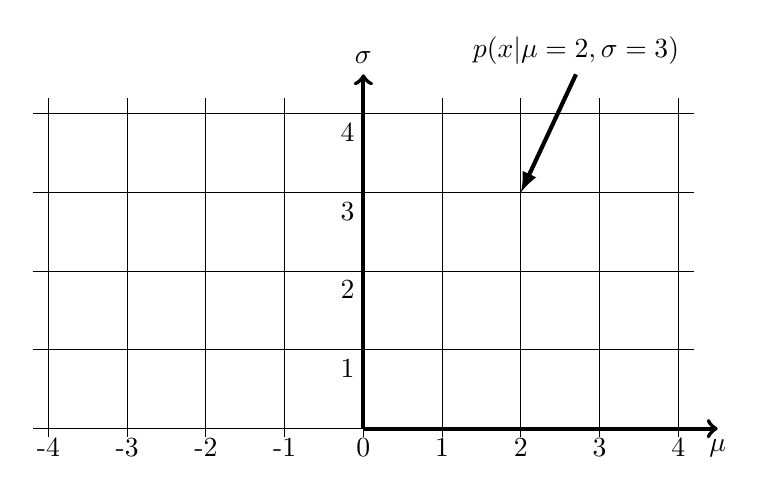
\begin{tikzpicture}
	% Draw horizontal lines
	\foreach \y in {0,1,2,3,4}
	\draw (-4.2,\y) -- (4.2,\y);
	
	% Draw vertical lines
	\foreach \x in {-4,-3,-2,-1,0,1,2,3,4}
	\draw (\x,0) -- (\x,4.2);
	
	% Draw x and y axes
	\draw[thick, ->, line width=1.5pt] (0,0) -- (4.5,0) node[below] {$\mu$};
	\draw[thick, ->, line width=1.5pt] (0,0) -- (0,4.5) node[above] {$\sigma$};
	
	% Label tick marks
	\foreach \x in {-4,-3,-2,-1,0,1,2,3,4}
	\draw (\x,-0.1) -- (\x,0.1) node[below=3pt] {\x};
	\foreach \y in {1,2,3,4}
	\draw (0,\y) -- (-0.2,\y) node[below] {\y};
	
	\draw[thick, ->, >= latex, line width=1.5pt] (2.7,4.5) -- (2,3);
	\node at (2.7,4.5) [above] {$p(x|\mu = 2,\sigma = 3)$};
		
\end{tikzpicture}
\caption{This figure illustrates the manifold of normal distributions. As coordinate system, $\mu$ and $\sigma$ are used. Every point in this manifold represents a probability distribution, as indicated by the arrow. \label{fig:NormalDistributionManifold}}
\end{figure}
It might also be clear that the coordinate system of a manifold is definable in multiple different ways. Although it's always given in our use case, let's therefore denote that in general when we have coordinates $\theta$ we also need a mapping $\phi$, which maps coordinates to points on a manifold. This means that by applying $\phi(p)$ to a point $p\in S$ the resulting vector in $\mathbb{R}^n$ resembles the coordinates of that point. We can also apply the inverse of that mapping to a set of coordinates to the point in the manifold that's represented by those coordinates.
%Now we need to introduce some assumptions for the following theorems and definitions:
%\begin{enumerate}
%	\item All $p(x|\theta)$ must have a common "support" $X$ so that $p(x|\theta)>0$ for all $x\in X$.
%	\item Let's define $\ell(x|\theta)$ = $\log p(x|\theta)$. For every fixed $\theta$, the $n$ functions $\partial/\partial \theta_i \ell(x|\theta)$ labeled by $i$ have to be linearly independent. We will later see that $\ell$ here corresponds to the $\ell$ of the loss function if we consider the manifold of a machine learning network.
%	\item The moments of random variables $\partial/\partial \theta_i \ell(x|\theta)$ exist up to necessary orders. 
%	\item The partial derivative $\partial/\partial\theta_i$ and the integration over the measure of $X$ can always be interchanged.
%\end{enumerate}

\subsection{Tangent space}
The tangent space $T_p$ of a manifold at point $p$ is a vector space obtained by linearization of the manifold around $p$. For intuition purposes, let's take a look at the tangent plane of a 2d-surface in \cref{fig:TangentSpacePlot}. Here the tangent space is simply a plane that touches the surface in one point, with derivatives adjusted to match the surface at that point.
\begin{figure}
	\centering
	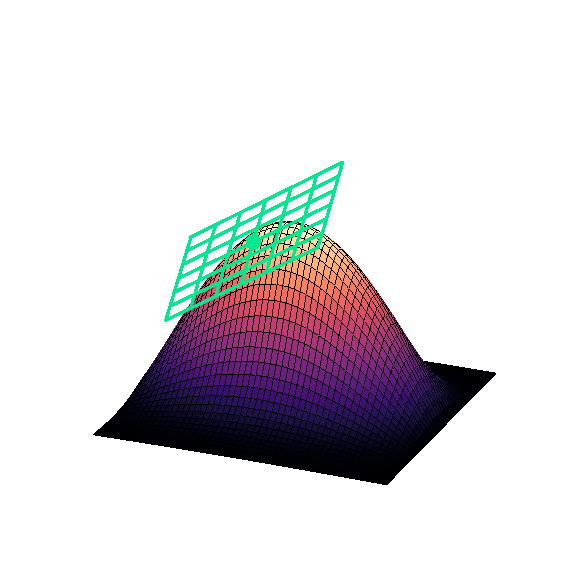
\includegraphics[width = 12cm, clip, trim= 0cm 1.5cm 0cm 2cm]{text/FisherInformation/plots/TangentSpacePlot.pdf}
	\label{fig:TangentSpacePlot}
	\caption{This figure contains an example of a tangent space of a manifold, which in this case is a 2d-surface.}
\end{figure}
For the general case of $n$-dimensional manifolds, it is obvious that tangent spaces aren't simply tangent planes of surfaces in every case, therefore let's introduce a way how to calculate a tangent space.\\
First we will define curves $c(t)$ that are continuous mappings from an interval $[a,b] \in \mathbb{R}$ into the manifold $S$. In the parametric representation, the curve is given by $\theta(t)$. Now we can define what a tangent vector is.\\
Imagine a smooth real function $f(\theta): S \rightarrow \mathbb{R}$. We can now restrict this function to our predefined curve $c$ by $f \circ c : [a,b] \rightarrow \mathbb{R}$. We'll denote this via $f\left(\{\theta(t)\}\right)$ in the coordinate expression. The derivative $Cf$ of this function is then given by 
\begin{equation}
	Cf = \tAbl{f\circ c}{t} = \sum_{i=1}^{n} \pAbl{f}{\theta_i}\tAbl{\theta_i(t)}{t} = \underbrace{\left(\sum_{i=1}^{n}\tAbl{\theta_i}{t}\pAbl{}{\theta_i}\right)}_{\text{Operator }C} f.
\end{equation}
Therefore we can associate a directional derivative operator $C$ with each curve. The only dependence of this operator regarding the curve is $\tAbl{\theta_i}{t}$, where we might also clarify that this derivative depends itself on the point where it is calculated at.\\
If the manifold is infinitely differentiable, the set of these mappings $C$ at a fixed point on the manifold forms a $n$-dimensional vector space, called the "\textbf{tangent space}" $T_p$ of that point $p$. \\
To make this more clear, let's look at the simplest basis for this vector space, which we'll call the "natural basis" of the tangent space. For this we'll consider curves $c_1,c_2, \dotsc c_n$ through a point $p_0$, where the curves are defined as 
\begin{equation}
	c_i(t) = \{\theta_1^0,\theta_2^0, \dotsc, \theta_i^0 + (t-t_0), \dotsc \theta_n^0 \},
\end{equation}
so that $c_i(t_0) = \{\theta_1^0,\theta_2^0, \dotsc\theta_n^0\} = p_0$ for every curve. The tangent vectors $C_i$ then are simply the derivatives regarding their corresponding coordinate $C_i f = \partial/\partial \theta_i f$. We will denote this in short by $C_i = \partial_i$. The $n$ vectors $\partial_i$ are linearly independent and form the natural basis for the tangent space. This means that any tangent vector $A$ can be represented by 
\begin{equation}
	A = \sum_{I=1}^{n} A_i \partial_i,
\end{equation}
with components with respect to the natural basis $A_i$. If we are given a curve $c(t)$ going through $c(t_0)$ which derivative operator $C$ in $t_0$ is equivalent to the vector $A$, we can find the natural basis representation of $A$ as
\begin{equation}
	A_i = \left. \tAbl{\theta_i}{t}\right|_{t_0}.
\end{equation} \\
Now let's take a look at the case of manifolds of statistical models. First we will define $\ell$ as
\begin{equation}
	\ell(x|\theta) = \log f(x|\theta),
\end{equation}
and assume that for fixed $\theta$, the $n$-functions $\partial_i \ell(x|\theta)$ are linearly independent. This means that we can construct a vector space by defining
\begin{equation}
	T_\theta^{(1)} = \{A(x) | A(x) = A_i \partial_i \ell(x|\theta)\}.
\end{equation}
We do this because there is a natural isomorphism between the tangent space $T_\theta$ and this space $T_\theta^{(1)}$ through 
\begin{equation}
	\partial_i \in T_\theta \leftrightarrow \partial_i \ell(x|\theta) \in T_\theta^{(1)}.
\end{equation}
We will call $T_\theta{(1)}$ the "\textbf{1-representation}" of our tangent space for the statistical models. We will now use this vector to define an inner product on the tangent space and it's 1-representation.\\
\subsection{Riemannian metric and Fisher Information}
When the inner product of the tangent spaces $T_p$ is defined, the manifold is called a \textbf{Riemannian manifold}.\\
Let's first consider the inner product of the 1-representation space. Let $A(x)$ and $B(x)$ be 1-representations of $A$ and $B \in T_\theta$. It is intuitive to define the inner product as 
\begin{equation}
	\langle A(x), B(x) \rangle = \underset{x\in X}{E} \Big[A(x) B(x)\Big],
\end{equation}
with the expectation value $E[\cdot]$. Since the tangent space is isomorphic to its 1-representation, the inner product also translates via 
\begin{equation}
	\langle A, B \rangle = \langle A(x),B(x) \rangle.
\end{equation}
This also means that we can calculate the inner product of the basis vectors as 
\begin{equation}
	\begin{split}
		g_{ij}(\theta) \vcentcolon= \langle \partial_i, \partial_j\rangle = \langle \partial_i\ell(x|\theta), \partial_j\ell(x|\theta)\rangle \\
		= \underset{x \in X}{E} \Big[\partial_i\ell(x|\theta), \partial_j\ell(x|\theta)\Big].
	\end{split}
\end{equation}
The resulting object $g_{ij}(\theta)$ is called the \textbf{Riemannian metric tensor} of the manifold. We can see that the Riemannian metric tensor for the statistical model is equivalent to the Fisher Information. It might be of interest to note here that we assume that $\ell$ only depends explicitly on $\theta$. If we denote these as implicit dependencies, we have to replace the partial derivatives with absolute ones.\\
The inner product of two vectors can now be expressed with the metric tensor as
\begin{equation}
	\langle A,B \rangle = \sum_{i,j} A_iB_jg_{ij}(\theta)
\end{equation}
in the component form. \\
Using this representation of the inner product, we can define various things. For example, the length of a vector $A$ is defined as $|A|^2 = \sum_{i,j} A_iA_j g_{ij}$, the orthogonality of two vectors when their inner product is zero, and the distance between two points $\theta^{(0)}$ and $\theta^{(1)}$ along the curve $c$ is defined by 
\begin{equation}
	s = \int_{t_0}^{t_1} \sum_{i,j} \sqrt{g_{ij}\tAbl{\theta_i}{t}\tAbl{\theta_j}{t}} \mathrm{d}t. 
\end{equation}
This also introduces the concept of \textbf{Riemannian geodesics}. These are the curves that connect two points via the minimal distance between the two.\\
Another representation of the metric tensor or the FI is 
\begin{equation}\label{eq:SecondRepresentationOfFisherInfo}
	g_{ij}(\theta) = - \underset{x\in X}{E} \Big[ \partial_i \partial_j \ell(x|\theta) \Big].
\end{equation}
A proof of this is denoted in \cref{sec:ProofForeq:SecondRepresentationOfFisherInfo}.

\subsection{Scalar curvature and Christoffel symbols}
Here we will only give the definitions needed to compute the scalar curvature of a statistical manifold. A full understanding requires much more mathematics than we will go over here. If you are interested in this, please see \cite{AmarisLectureNotes} and \cite{GeneralRelativityBook}.\\
We will use Einstein notation for these equations. First we define the Christoffel-symbols which can be calculated from the Riemannian metric via
\begin{equation}
	\Gamma^{i}_{jk} = \frac{1}{2}g^{im} \left(\pAbl{g_{mk}}{\theta_l} + \pAbl{g_{ml}}{\theta_k} - \pAbl{g_{kl}}{\theta_m}\right),
\end{equation} 
where $g^{ij} = (g^{-1})_{ij}$ are the components of the inverse of the metric.
From those we can define the Riemannian curvature tensure as 
\begin{equation}
	R^{i}_{jkl} = \partial_k \Gamma^i_{jl} - \partial_l \Gamma^i_{jk} + \Gamma^i_{mk}\Gamma^m_{jl} - \Gamma^i_{ml}\Gamma^m_{jk}.
\end{equation}
Now we can finally state the scalar Ricci curvature as 
\begin{equation}
	R = g^{ij} R^m_{imj}.
\end{equation}